\documentclass[../distribution_theory_notes.tex]{subfiles}
\begin{document}
\section{Aula 09 - 20 de Setembro, 2024}
\subsection{Motivações}
\begin{itemize}
 \item Existência e Regularidade das Convoluções;
 \item Resultados de Densidade; 
 \item Lema de Uryhson \(\mathcal{C}_{c}^{\infty}\).
\end{itemize}
\subsection{Propriedades das Convoluções I}
  Para contextualizar, tudo o que disser respeito à ``mensurabilidade'' será no sentido de Borel para conjuntos e funções, e ``dx, dy, dz'' todos indicarão a medida de Lebesgue na \(\sigma \)-álgebra \(\mathcal{B}_{\mathbb{R}^{n}}\) correspondente.
   \begin{tcolorbox}[
   skin=enhanced,
   title=Observação,
   fonttitle=\bfseries,
 colframe=black,
   colbacktitle=cyan!75!white, 
   colback=cyan!15,
   colbacklower=black,
 coltitle=black,
   drop fuzzy shadow,
   %drop large lifted shadow
   ]
   Se f é mensurável em \(\mathbb{R}^{n}\), então o mapa 
     \[
       (x, y)\mapsto F(x, y)=f(x-y)
     \]
     é mensurável em \(\mathbb{R}^{n}\times \mathbb{R}^{n}\) (equipado com a \(\sigma \)-álgebra produto). O argumento para isso é notar que, definindo a função contínua 
    \begin{align*}
      S:&\mathbb{R}^{n}\times \mathbb{R}^{n}\rightarrow \mathbb{R}^{n}\\ 
        &(x, y)\mapsto S(x, y)=x-y,
    \end{align*}
    podemos então escrever 
      \[
        F = f\circ s,
      \]
      donde segue que, se U é um aberto de \(\mathbb{R}^{n}\),
        \[
          F^{-1}(U)=S^{-1}(\underbrace{f^{-1}(U)}_{\in \mathcal{B}_{\mathbb{R}^{n}}}) 
        \]
        e S é \((\mathcal{B}_{\mathbb{R}^{n}\times \mathbb{R}^{n}}, \mathcal{B}_{\mathbb{R}^{n}})\)-mensurável.

        Em particular, fixado um vetor x de \(\mathbb{R}^{n}\), o mapa \(y\mapsto f(x-y)\) ser mensurável resulta em 
          \[
            y\mapsto f(x-y)g(y)
          \]
          também sendo sempre que \(g\) o for, justificando a integração na definição seguinte.
   \end{tcolorbox}
  \begin{def*}
    Sejam f e g mensuráveis em \(\mathbb{R}^{n}\). Dado um vetor \(x\in \mathbb{R}^{n}\), o \textbf{produto de convolução de f por g em x} é dado por 
      \[
        f*g(x)=\int_{}^{}f(x-y)g(y) \mathrm{dy},
      \]
      sempre que a integral existir. \(\square\)
  \end{def*}
 \begin{lemma*}
   Supondo que todas as integrais a seguir existam, temos: 
  \begin{align*}
    &(i)\;f*g = g*f; \text{ (comutatividade)} \\
    &(ii)\;f*(g*h) = (f*g)*h; \text{ (associatividade)}\\
    &(iii)\;f*(g+h) = f*g + f*h; \text{ (distributividade)}\\
    &(iv)\; T_hf(x)\coloneqq f(x-h) \Rightarrow T_h(f*g)=(T_hf)*g=f*(T_hg).
  \end{align*}
  Além disso, (v) se F e G são fechados de \(\mathbb{R}^{n}\) tais que \(f=0\) em quase todo ponto de \(\mathbb{R}^{n}\setminus{F}\) e \(g=0\) em quase todo ponto de \(\mathbb{R}^{n}\setminus{G},\) então \(f*g=0\) em quase todo ponto de \(\mathbb{R}^{n}\setminus{(\overline{F+G})}\); em outras palavras, 
    \[
      \mathrm{supp}(f*g)\subseteq \overline{\mathrm{supp}(f)+\mathrm{supp}(g)}.
    \]
 \end{lemma*}
\begin{proof*}
  (i) É uma consequência direta do Teorema de Mudanças de Variáveis: fazendo \(h(z)=x-z\) em 
    \[
      \int_{h(A)}^{}F(y) \mathrm{dy}=\int_{A}^{}(F\circ h)(z) |\det{h'(z)}|\mathrm{dz},
    \]
    temos 
      \[
        f*g(x)=\int_{}^{}f(x-y)g(y) \mathrm{dy} = \int_{}^{}f(z)g(x-z) \mathrm{dz}=g*f(x).
      \]

      (ii) Segue do \hyperlink{fubini_tonelli}{\textit{Teorema de Fubini}} da seguinte forma: 
     \begin{align*}
       [f*(g*h)](x) = \int_{}^{}f(x-y)[g*h(y)] \mathrm{dy} &= \int_{}^{}f(x-y)\biggl[\int_{}^{}g(y-z)h(z) \mathrm{dz}\biggr] \mathrm{dy}\\ 
                                                           &= \int_{}^{}\biggl[\int_{}^{}f(x-y)g(y-z) \mathrm{dy}\biggr] h(z)\mathrm{dz}\\ 
                                                           &= \int_{}^{}\biggl[\int_{}^{}f(w)g(x-w-z) \mathrm{dw}\biggr]h(z) \mathrm{dz}\\ 
                                                           &= \int_{}^{}(f*g)(x-z)h(z) \mathrm{dz}  = [(f*g)*h](x),
     \end{align*}
     onde foi utilizada a mudança de variáveis de z para w pela forma 
       \[
         H(w)=x-w,\quad w\in \mathbb{R}^{n}.
       \]

       (iii) Exercício.

       (iv) Com efeito, pela própria definição de convolução, 
      \begin{align*}
        [T_h(f*g)](x)=f*g(x-h) &= \int_{}^{}f(x-h-y)g(y) \mathrm{dy}\\ 
                               &= \int_{}^{}(T_hf)(x-y)g(y) \mathrm{dy}\\ 
                               &= [(T_hf)*g](x),
      \end{align*}
      e a outra igualdade segue aplicando o item (i), ou seja, por comutação.

      (v) Devemos mostrar que, se x não pertence a \(F+G\), então \(F\cap (x-G)=\emptyset \) e, consequentemente, \(f*g(x)=0\). Com efeito, caso contrário, existiria z em \(F\cap (x-G)\), ou seja, z é tanto um membro de F quanto pode ser escrito como \(z=x-w\), onde \(w\in G\). Assim, \(x=z+w\), com z em F e w em G, uma contradição à escolha de x. Logo, \(x\in \mathbb{R}^{n}\setminus{(F+G)}\), resultando em 
        \[
          f*g(x)=0
        \]
        e, portanto, se \(f*g\) for contínua, teremos \(\mathrm{supp}(f*g)\subseteq \overline{F+G}.\) \qedsymbol
    \end{proof*}

  Para a existência e regularidade da convolução, comecemos com o seguinte lema: 
 \begin{lemma*}
   Se \(\varphi \in \mathcal{C}_{c}^{\infty}(\mathbb{R}^{n})\) e \(f\in L_{\mathrm{loc}}^{1}(\mathbb{R}^{n})\), então: 
  \begin{itemize}
    \item[i)] A convolução \(\varphi * f(x)\) existe para todo x em \(\mathbb{R}^{n}\), com 
      \[
        |\varphi *f(x)| \leq \Vert \varphi  \Vert_{\infty} \int_{x-K}^{}|f(y)| \mathrm{dy},\quad \forall x\in \mathbb{R}^{n}; \text{ e}
      \]
      \item[ii)] A convolução \(\varphi *f(x)\) pertence a \(\mathcal{C}^{\infty}(\mathbb{R}^{n})\), com 
        \[
          \partial^{\alpha }(\varphi *f)=(\partial^{\alpha }\varphi )*f,\quad \forall \alpha \in \mathbb{Z}_{+}^{n}.
        \]
  \end{itemize}
 \end{lemma*}
\begin{proof*}
  (i) Com efeito, dado x em \(\mathbb{R}^{n}\), se \(x-y\nin K\coloneqq \mathrm{supp}(\varphi )\) (ou, equivalentemente, \(y\not\in x-K\)), então 
    \[
      \varphi (x-y)=0 \Rightarrow \varphi (x-y)f(y)=0.
    \]
    Por outro lado, se y pertence a \(x-K\), então 
      \[
        |\varphi(x-y) f(y) | \leq \Vert \varphi  \Vert_{\infty} |f(y)|,
      \]
      donde segue que 
        \[
          y\mapsto \varphi (x-y)f(y)
        \]
        é integrável sobre \(x-K\), pois \(f\in L^{1}(x-K)\); consequentemente, 
          \[
            \varphi *f(x)=\int_{x-K}^{}\varphi (x-y)f(y) \mathrm{dy}=\int_{\mathbb{R}^{n}}^{}\varphi (x-y)f(y) \mathrm{dy}
          \]
          existe, com 
            \[
              |\varphi *f(x)|\leq \Vert \varphi  \Vert_{\infty} \int_{x-K}^{}|f(y)| \mathrm{dy},\quad \forall x\in \mathbb{R}^{n},
            \]
            terminando a prova da existência.

            (ii) Este item é uma consequência do teorema da convergência dominada de Lebesgue. Começando pela continuidade, seja 
            \[
            x_{j}\substack{\mathbb{R}^{n} \\ \longrightarrow \\ x_{0}}
            \]
            e definamos: 
              \[
                L\coloneqq \{x_{j}:\; j=0,1,2,\dotsc \}-K,
              \]
              que é compacto com \(\varphi (x_{j}-y)=0\) se y não pertence ao L, para todo j, tendo em vita que 
                \[
                  L=\bigcup_{j=0}^{\infty}(x_{j}-K)\Rightarrow \mathbb{R}^{n}\setminus{L}\subseteq \bigcap_{j=0}^{\infty}\mathbb{R}^{n}\setminus{(x_{j}-K)}\Rightarrow \varphi (x_{j}-y)=0
                \]
                sempre que y não pertence a L. Disto, obtemos 
                  \[
                    \varphi *f(x_{j})=\int_{L}^{}\varphi (x_{j}-y)f(y) \mathrm{dy},\quad \forall j=0,1,2,\dotsc .
                  \]
                  Como, para todo y em L, 
                    \[
                      \varphi (x_{j}-y)f(y)\substack{ \\ \longrightarrow \\ j\to\infty}\varphi (x_{0}-y)f(y)
                    \]
                    por conta da continuidade de \(\varphi \) e como 
                      \[
                        |\varphi (x_{j}-y)f(y)|\leq \Vert \varphi  \Vert_{\infty}|f(y)|,\quad \forall y\in L,\; f\in L^{1}(L),
                      \]
                      o teorema da convergência dominada permite concluirmos que 
                        \[
                          \lim_{j\to \infty}\varphi *f(x_{j})=\lim_{j\to \infty}\int_{L}^{}\varphi (x_{j}-y)f(y) \mathrm{dy}=\int_{L}^{}\varphi (x_{0}-y)f(y) \mathrm{dy}=\varphi *f(x_{0})
                        \]
                        e, logo, \(\varphi *f\) é contínua em qualquer \(x_{0}\) de \(\mathbb{R}^{n}\), mostrando que \(\varphi *f\in \mathcal{C}(\mathbb{R}^{n})\). 

                        A diferenciabilidade é provada de maneira análoga e usando indução, observando que, para \(x_{0}\in \mathbb{R}^{n}\), fixando \(j=1,2,\dotsc ,n\) e um \(\delta >0\) qualquer, temos: 

                        (I) Quando \(y\not\in \overline{B}(x_{0}; \delta  )-K\), 
                          \[
                            \frac{\partial^{}\varphi }{\partial x_{j}^{}}(x-y)f(y)=0,\quad \forall x\in \overline{B}(x_{0}; \delta ).
                          \]
                          Logo, se \(R\coloneqq \overline{B}(x_{0}; \delta )-K\), então 
                            \[
                              \biggl\vert \frac{\partial^{\varphi }}{\partial x_{j}^{}}(x-y)f(y) \biggr\vert \leq \biggl\Vert \frac{\partial^{}\varphi }{\partial x_{j}^{}} \biggr\Vert_{\infty}|f(y)|,\quad \forall y\in R,
                            \]
                            com f em \(L^{1}(R)\), mostrando que o segundo termo é uma função g em \(L^{1}(R)\).

                            (II) Além do que foi dito em (I), 
                              \[
                                \varphi *f(x)=\int_{R}^{}\varphi (x-y) \mathrm{dy}
                              \]
                              e, para todo x em \(\overline{B}(x_{0}; \delta )\), 
                                \[
                                  \biggl(\frac{\partial^{}\varphi }{\partial x_{j}^{}}\biggr)* f(x) = \int_{R}^{}\biggl(\frac{\partial^{}\varphi }{\partial x_{j}^{}}(x-y)\biggr)f(y) \mathrm{dy}.
                                \]

                                Assim, juntando (I) e (II), temos as condições para aplicar a derivada sob o sinal de integração via convergência dominada, nos dando 
                                  \[
                                    \frac{\partial^{}}{\partial x_{j}^{}}(\varphi *f)(x_{0})=\int_{R}^{}\biggl(\frac{\partial^{}\varphi }{\partial x_{j}^{}}(x_{0}-y)\biggr)f(y) \mathrm{dy},
                                  \]
                                  que, pela segunda parte do (II), é exatamente \(\biggl(\frac{\partial^{}\varphi }{\partial x_{j}^{}}\biggr)* f(x)\). Pela arbitrariedade de \(x_{0}\in \mathbb{R}^{n}\), resulta que existe a derivada \(\frac{\partial^{}}{\partial x_{j}^{}}(\varphi *f)\) para todo j, e, como \(\mathrm{supp}\biggl(\frac{\partial^{}\varphi }{\partial x_{j}^{}}\biggr)\) está contido em \(\mathrm{supp}(\varphi )\), a continuidade d derivada também está garantida, ou seja, \(\varphi *f\in \mathcal{C}^{1}\). Para as próximas derivada, basta reiterar este processo, portanto provando o lema. \qedsymbol
                                    
\end{proof*}
  \begin{tcolorbox}[
  skin=enhanced,
  title=Observação,
  fonttitle=\bfseries,
colframe=black,
  colbacktitle=cyan!75!white, 
  colback=cyan!15,
  colbacklower=black,
coltitle=black,
  drop fuzzy shadow,
  %drop large lifted shadow
  ]
  Se \(\varphi \in \mathcal{C}_{c}^{\infty}(\mathbb{R}^{n})\) e \(f\in \mathcal{C}^{m}(\mathbb{R}^{n})\), desde que \(|\alpha |\leq m,\) então 
    \[
      \partial^{\alpha }(\varphi*f)=\varphi *(\partial^{\alpha }f).
    \]
  \end{tcolorbox}

  Este lema será usado para provar a densidade de \(\mathcal{C}_{c}^{\infty}(\Omega )\) em diversos espaços de funções, tal como no 
 \begin{theorem*}
   O espaço \(\mathcal{C}_{c}^{\infty}(\Omega )\) é denso em \(\mathcal{C}(\Omega )\) segundo a convergência uniforme em compactos. 
 \end{theorem*}
 Antes de demonstrá-lo, precisamos do \hyperlink{uryhson_lemma}{\textit{Lema de Uryhson \(\mathcal{C}_{c}^{\infty}\)}}: 
 \hypertarget{uryhson_lemma}{
   \begin{theorem*}[Lema de Uryhson \(\mathcal{C}_{c}^{\infty}\)]
    Seja K um compacto contido em \(\Omega \). Existe \(\psi \in \mathcal{C}_{c}^{\infty}(\Omega )\) com \(\psi \equiv 1\) uma vizinhança de K e \(0\leq \psi \leq 1\).
  \end{theorem*}
 }
 \begin{proof*}
   Começamos fixando \(\varphi \in \mathcal{C}_{c}^{\infty}(\mathbb{R}^{n})\) com \(\varphi \geq 0,\; \mathrm{supp}(\varphi )=\overline{B}(0;1)\) e 
     \[
       \int_{}^{}\varphi = 1.
     \]
     Como exemplo de função que satisfaça tudo isso, temos a \(\varphi_{0}\in \mathcal{C}_{c}^{\infty}(\overline{B}(0;1))\) que apresentamos antes; aí, para garantir a integral unitária, fazemos 
       \[
         \varphi \coloneqq \frac{1}{c_{0}}\varphi_{0},\quad c_{0}= \int_{}^{}\varphi_{0}.
       \]

       Para cada \(\varepsilon >0\), seja \(\varphi_{\varepsilon }(x)\coloneqq \varepsilon^{-n}\varphi(x/\varepsilon )\), onde x é um vetor de \(\mathbb{R}^{n}\). 
      \begin{figure}[H]
      \begin{center}
      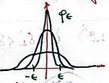
\includegraphics[height=0.5\textheight, width=0.5\textwidth, keepaspectratio]{./Images/phi_epsilon_09.png}
      \end{center}
      \caption{conforme \(\varepsilon \) tende ao 0 pela direita, o valor da \(\varphi \) se aproxima de infinito: \(\lim_{\varepsilon \to 0^{+}}\varphi_{\varepsilon }(0)=\lim_{\varepsilon \to 0^{+}}\frac{1}{\varepsilon^{n}}=\infty.\)}
      \end{figure}

       Observe que: 
      \begin{align*}
        &(a)\; \varphi_{\varepsilon }\in \mathcal{C}_{c}^{\infty}(\mathbb{R}^{n}); \\
        &(b)\; \mathrm{supp}(\varphi_{\varepsilon })=\overline{B}(0; \varepsilon );\\
        &(c)\; \varphi_{\varepsilon }\geq 0; \text{ e}\\
        &(d)\; \int_{}^{}\varphi_\varepsilon(x) \mathrm{dx}=\int_{}^{}\varepsilon^{-n}\varphi \biggl(\frac{x}{ \varepsilon }\biggr) \mathrm{dx} \underbrace{=}_{\mathclap{h(y)=\varepsilon y;\; \det{h'(y)}=\varepsilon^{n}}} \int_{}^{}\varphi (y) \mathrm{dy}.
      \end{align*}

      Além disso, fixemos \(\delta_{0}>0\) com \(\delta_{0}< d(K, \partial \Omega )\), porque \(K\cap \partial \Omega =\emptyset \) com K compacto e \(\partial \Omega \) fechado, e consideremos o conjunto 
        \[
          K_{0}=\{x\in \Omega :\; d(x, K)\leq \delta_{0}\} = \bigcup_{a\in K}^{}\overline{B}(a; \delta_{0}),
        \]
        o qual está contido em \(\Omega \) e contém o K.
       \begin{figure}[H]
       \begin{center}
       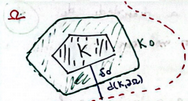
\includegraphics[height=0.5\textheight, width=0.5\textwidth, keepaspectratio]{./Images/delta_from_k_09.png}
       \end{center}
       \caption{o K é o conjunto dos pontos de \(\Omega \) a uma distância não maior que \(\delta_{0}\) do conjunto K.}
       \end{figure}

       Agora, consideremos também \(f=\chi_{K_{0}}\); note que 
       \[
         f\in L^{1}(\mathbb{R}^{n})\hookrightarrow L_{\mathrm{loc}}^{1}(\mathbb{R}^{n}),
         \]
         donde, para todo \(\varepsilon >0\), 
           \[
             \varphi_{\varepsilon }*f\in \mathcal{C}^{\infty}(\mathbb{R}^{n}).
           \]
           Expandindo a conta da convolução de \(\varphi_\varepsilon \) com f, segue o seguinte: 
          \begin{align*}
            \varphi_\varepsilon *f(x)=\int_{}^{}\varphi_\varepsilon (x-y)f(y) \mathrm{dy}&= \int_{K_{0}}^{}\varphi_\varepsilon (x-y)f(y) \mathrm{dy}\\ 
                                                                                         &= \int_{K_{0}}^{}\varphi_\varepsilon (x-y) \mathrm{dy}\\ 
                                                                                         &= \int_{K_{0}\cap (x-B_\varepsilon (0))}^{}\varphi_\varepsilon (x-y) \mathrm{dy}.
                                                                                     
          \end{align*}
          pois \(\mathrm{supp}(\varphi_\varepsilon )=\overline{B}(0;\varepsilon =bbB(0; \varepsilon ))\). Logo, \(x-y\) não pertence à bola fechada \(\overline{B}_\varepsilon (0)\), o que resulta em \(\varphi_\varepsilon (x-y)=0\), ou seja, 
            \[
              y\not\in \overline{B}(0; \varepsilon )\Rightarrow \varphi_\varepsilon (x-y)=0.
            \]
            Agora, basta diminuir \(\varepsilon \) o suficiente! Para começar, como uma ``etapa zero'', repare que podemos dar continuidade às formas equivalentes à convolução acima de onde paramos: 
              \[
                \varphi_\varepsilon *f(x)=\int_{K_{0}\cap (x-)\overline{B}(0; \varepsilon )}^{}\varphi_\varepsilon (x-y) \mathrm{dy} = \int_{K_{0}\cap \overline{B}(x; \varepsilon )}^{} \varphi_\varepsilon (x-y)\mathrm{dy},
              \]
              tal que, se \(B_\varepsilon (x)\) for um subconjunto de \(K_{0}\), teremos 
                \[
                  \varphi_\varepsilon *f(x)=\int_{\overline{B}(x; \varepsilon )}^{}\varphi_\varepsilon (x-y) \mathrm{dy}=1.
                \]
                Com respeito ao primeiro passo, diminuiremos \(\varepsilon \) a fim de garantir a compacidade de \(\mathrm{supp}(\varphi_\varepsilon *f)\) e a continência dele em \(\Omega \). Note que, se \(\delta_0<\delta_1<d(x, \mathbb{R}^{n}\setminus{\Omega }) \), então 
                  \[
                    K_1\coloneqq \bigcup_{a\in K}^{}\overline{B}(a;\delta_1)
                  \]
                  é tal que \(K_{0}\subseteq K_1\subseteq \Omega \) pelo mesmo raciocínio usado para \(K_{0}\). 
                 \begin{figure}[H]
                 \begin{center}
                 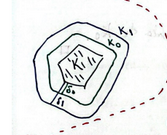
\includegraphics[height=0.5\textheight, width=0.5\textwidth, keepaspectratio]{./Images/covering_k_09.png}
                 \end{center}
                 \caption{o \(K_1\) agora se situa entre \(K_0\) e \(\Omega\).}
                 \end{figure}

                 Também, x não pertence a \(K_1\), tendo em vista que \(d(\mathbb{R}^{n}\setminus{K}, K)\geq \delta_1\), do que segue que, quando \(0<\varepsilon <\delta_1-\delta_0,\)
                   \[
                     \varphi_\varepsilon *f(x)=0,
                   \]
                   pois 
                     \[
                       K_{0}\cap (x-\overline{B}(0; \varepsilon ))=\emptyset;
                     \]
                     caso contrário, se \(y\in K_{0}\cap (x-\overline{B}(0; \varepsilon ))\), então \(y\in K_{0}\) e \(y=x-z\) com \(|z|\leq \varepsilon \), que resultaria em 
                       \[
                         |y-a|\leq \delta_{0}
                       \]
                       para algum \(a\in K\). Logo, 
                         \[
                           |x-a|\leq |x-y|+|y-a|\leq |z|+\delta_{0}\leq \varepsilon +\delta_{0}<(\delta_1-\delta_0)+\delta_0=\delta_1,
                         \]
                         que contradiz o fato de x não pertencer a \(K_1\) a partir do momento que isto requer que \(d(x, a)>\delta_1\) para todo a em K. Isto mostra duas coisas: que \(0<\varepsilon <\delta_1-\delta_0\), tal que \(\mathrm{supp}(\varphi_\varepsilon *f)\) é um compacto contido em \(K_1\), e que, consequentemente, 
                           \[
                             \varphi_\varepsilon *f\in \mathcal{C}_{c}^{\infty}(\Omega ).
                           \]

                           Quanto ao segundo passo, queremos encontrar o aberto \(U\) de \(\Omega \) contendo K tal que 
                             \[
                               \varphi_\varepsilon *f\equiv 1
                             \]
                             em U. Para isso, precisamos escolher \(0<\varepsilon_0\) para o qual teremos 
                               \[
                                 x-\overline{B}_{\varepsilon_{0}}(0)\subseteq K_{0}
                               \]
                               com x em U. Ora, se a é um membro de K e \(y=x-z\in x-\overline{B}_{\varepsilon_{0} }(0)\), onde \(|z|\leq \varepsilon_{0}\), então 
                                 \[
                                   |y-a|\leq |x-a|+|z|\leq |x-a|+\varepsilon_{0} \leq \delta_{0},
                                 \]
                                 o qual pode ser obtido tomando 
                                   \[
                                     U\coloneqq \bigcup_{a\in K}^{}B(a; \varepsilon_{0})
                                   \]
                                   se \(2\varepsilon_{0}=\delta_{0}\). Logo, com este \(\varepsilon_{0}\), caso x pertença a U, seguirá que 
                                     \[
                                       x-\overline{B}_{\varepsilon_{0}}(0)\subseteq K_{0}\Rightarrow (\varphi_{\varepsilon_{0}}*f)(x)=\int_{x-\overline{B}_{\varepsilon }(0)}^{}\varphi_{\varepsilon }(x-y) \mathrm{dy}=\int_{|z|\leq \varepsilon }^{}\varphi_{\varepsilon }(z) \mathrm{dz}=1.
                                     \]

                                     Portanto, 
                                       \[
                                         0<\varepsilon <\min\limits_{}\biggl\{\frac{\delta_{0}}{2}, \delta_1-\delta_0\biggr\} \Rightarrow \psi \coloneqq \varphi_\varepsilon *f\in \mathcal{C}_{c}^{\infty}(\Omega )
                                       \]
                                       e \(\psi\equiv 1\) em \(U=\bigcup_{a\in K}^{}B(a; \varepsilon )\subseteq \Omega \), com 
                                         \[
                                           0\leq \psi (x)=\int_{}^{}\varphi_\varepsilon (x-y)f(y) \mathrm{dy}\leq \int_{}^{}\varphi_\varepsilon (x-y) \mathrm{dy}=1,
                                         \]
                                         pois, sendo f a característica de \(K_{0}\), temos \(0\leq f\leq 1\), finalizando a prova. \qedsymbol 

                             \end{proof*}

                              \begin{tcolorbox}[
                              skin=enhanced,
                              title=Observação,
                              fonttitle=\bfseries,
                            colframe=black,
                              colbacktitle=cyan!75!white, 
                              colback=cyan!15,
                              colbacklower=black,
                            coltitle=black,
                              drop fuzzy shadow,
                              %drop large lifted shadow
                              ]
                              A topologia limite indutivo em \(\mathcal{C}_{c}^{\infty}(\Omega )\) \textit{não é metrizável}! Com efeito, seja d uma métrica em \(\mathcal{C}_{c}^{\infty}(\Omega )\) tal que 
                                \[
                                  \varphi_{j}\substack{\mathcal{C}_{c}^{\infty}(\Omega ) \\ \longrightarrow \\ 0} \Longleftrightarrow d(\varphi_{j}, 0)\substack{ \\ \longrightarrow \\ j\to \infty}0.
                                \]
                                Dado um esgotamento \(\{K_{j}\}_{j}\) de \(\Omega \), podemos escolher, para cada j, \(\varphi_{j}\in \mathcal{C}_{c}^{\infty}(\Omega )\) com \(\varphi_{j}\equiv 1\) em \(K_{j}.\) Assim, fixado j, 
                                  \[
                                    \lim_{\varepsilon \to 0^{+}}\varepsilon \varphi_{j}=0
                                  \]
                                  em \(\mathcal{C}_{c}^{\infty}(\Omega )\). Portanto, escolhemos \(\varepsilon_{j}\) tal que 
                                    \[
                                      d(\varepsilon_{j}\varphi_{j}, 0)< \frac{1}{j},
                                    \]
                                    donde teremos 
                                      \[
                                        \varepsilon_{j}\varphi_{j}\to 0
                                      \]
                                      segundo d, mas não em \(\mathcal{C}_{c}^{\infty}(\Omega )\), pois 
                                        \[
                                          \bigcup_{j}^{}\mathrm{supp}(\varepsilon_{j}\varphi_{j})=\Omega 
                                        \]
                                        não é compacto.
                                
                              \end{tcolorbox}
 \subsection{Apêndices}
 \subsubsection{Consequências da Convergência Dominada}
 \subsubsection{Operadores Integrais}

\end{document}
